\documentclass[
  journal=largetwo,
  year=2023,
]{cup-journal}

\usepackage{amsmath}
\usepackage[nopatch]{microtype}
\usepackage{booktabs}
\usepackage[]{hyperref}
\usepackage{physics}


\title{Physical Implementation of Quantum Computers}

\author{Thiago Mattos}
\affiliation{Universidade Federal de Minas Gerais, Departamento de Física, Belo Horizonte, 31270-901, Minas Gerais, Brazil}
\email[T. Mattos]{thiagomattos@ufmg.br}

\author{Eric Botelho}
\affiliation{Universidade Federal de Minas Gerais, Departamento de Física, Belo Horizonte, 31270-901, Minas Gerais, Brazil}

\addbibresource{references.bib}

\keywords{quantum computer, superconducting qubits, ion trap, photonic model}

\begin{document}

\begin{abstract}
  This work aims to explain the physical principles of quantum computers. We will discuss how some physical systems can be used to peform computation, specialy with respect to three chosen impleentations, as well as the main advantages and disadvantages of each implementation.
  The implementations we will discuss are ion traps, photonic models and solid state systems. The ion trap model revolves around the manipulation of ions confined within a trap, while the photonic model centers on the manipulation of photons within a cavity, and the solid-state model focuses on the manipulation of electrons within a superconducting circuit.
  The main advantages and disadvantages of each model are presented, as well as the main challenges for the construction of a quantum computer.

\end{abstract}

\section{Introduction}

When delving into the realm of quantum computing, a crucial inquiry arises: Can a quantum computer truly be realized in the physical world? This article is devoted to the exploration and elucidation of the feasibility of physically implementing quantum computers. It aims to present various models of quantum computers while engaging in a concise discussion and general analysis of the subject matter.

Quantum computing possesses a remarkable attribute: its capacity to tackle computationally demanding tasks that surpass the capabilities of classical computers. Noteworthy quantum algorithms, such as Shor's algorithm for prime factorization and Grover's algorithm for searching unsorted databases, exemplify the potential of quantum computing in areas like cryptography, optimization, simulation, and machine learning.

Nonetheless, fully harnessing the power of quantum computing necessitates scalable implementations. Constructing large-scale quantum architectures presents substantial challenges due to the fragile nature of qubits and the imperative to preserve their quantum coherence, which can be easily disrupted by environmental disturbances.

In the race for scalable quantum computing, current leading implementations encompass photonics-based platforms, trapped ions, and superconducting circuits. Each approach possesses distinctive strengths and trade-offs. Of particular note are superconducting circuits, which have garnered significant attention owing to their ability to attain long qubit coherence times and facilitate the realization of multi-qubit gates.\autocite{arute_2019_quantum}.

While quantum computing remains in its early stages, progress in hardware development, error correction techniques, and algorithmic advancements holds the key to unlocking its transformative potential. As researchers and engineers strive to surmount the formidable challenges, quantum computing continues to captivate the scientific community and industry, offering a tantalizing glimpse into a future brimming with unparalleled computational capabilities.

In this work we will discuss the physical principles of quantum computers. We will discuss how some physical systems can be used to peform computation~\ref{sec:physical_properties}, specialy with respect to three chosen impleentations~\ref{cap:photonic}~\ref{cap:ion}~\ref{cap:superconductor}, as well as the main advantages and disadvantages of each implementation~\ref{sec:comparative}.


\section{Physical Propertires}
\label{sec:physical_properties}

The postulates of quantum mechanics serve as the foundational principles that underpin the theory's framework. Let us briefly delve into these fundamental postulates\autocite{cohentannoudji_1977_quantum}:

\begin{enumerate}[itemsep=5px]
  \item \emph{At a fixed time \(t_0\), the state of a physical system is defined by specifying a ket \(\ket{\psi(t_0)}\) belonging to the state space \(\mathcal{E}\)}

  \item \emph{Every measurable physical quantity \(\mathcal{A}\) is described by an operator \(A\) acting in \(\mathcal{E}\); this operator is an observable.}

  \item \emph{The only possible result of the measurement of a physical quantity \(\mathcal{A}\) is one of the eigenvalues of the corresponding observable \(A\).}

  \item \emph{When the physical quantity A is measured on a system in the normalized state \(\ket{\psi}\) the probability \(\mathcal{P}(a_n)\)  of obtaining the eigenvalue \(a_n\) of the corresponding observable A is: \\
          \( \mathcal{P}(a_n) = \sum_{i=1}^{g_n}\ket{\bra{u_n^i}\psi}|^2 \) \\
          where \(g_n\) is the degree of degeneracy of \(a_n\) and \( \{ \ket{u_n^i} \} \) \( (i=1,2,\ldots, g_n) \) is an orthonormal set of vectors in the eigensubspace \(\mathcal{E}_n\) associated with the eigenvalue \(a_n\) of A.}

  \item \emph{If the measurement of the physical quantity \(\mathcal{A}\) on the system in the state \(\ket{\psi }\) gives the result \(a_n\) the state of the system immediately after the measurement is the normalized projection, \(\frac{P_n\ket{\psi }}{\sqrt{\bra{\psi }P_n\ket{\psi }} }\), of \(\ket{\psi }\) onto the eigensubspace associated with \(a_n\).}

  \item \emph{The time evolution of the state vector \(|\psi (t)\) is governed by the Schrödinger equation: \\
          \(i\hbar \frac{d}{dt}\ket{\psi(t)} = H(t)\ket{\psi(t)}\) \\
          where \(H(t)\) is observable associated with the total energy of the system.}\label{post:schroedinger}
\end{enumerate}

\noindent \(H\) is called the {\it Hamiltonian operator} of the system, and it is the generator of time translations. The eigenvalues of \(H\) are the possible values of the total energy of the system, and the corresponding eigenvectors are the stationary states of the system.
The time evolution of the state vector \(\ket{\psi(t)}\) is governed by the Schrödinger equation, which is a linear differential equation. The solution of this equation can be encapsulated by the time evolution operator \(U(t,t_0)\), which is unitary and is given by:
\begin{align}
                   & U(t,t_0)       = e^{-iH(t-t_0)/\hbar}     \\
  \ket{\psi(t)}  = & U(t,t_0)\ket{\psi(t_0)}\label{eq:unitary}
\end{align}

\noindent In contemplating the utilization of quantum states for computational purposes, we discern that the temporal evolution, governed by an unitary operator, stands as the sole non-projective method for manipulating our state. Additionally, it is crucial to recognize the consequences of measuring the system, wherein the outcomes become confined to observables. The measurement process induces the collapse of the state into a subspace, thereby effectively destroying the previous information.

With the physical constraints imposed by quantum mechanics, we can now begin to discuss the prerequisites for the existance of a quantum computer, following the criteria established by DiVincenzo \autocite{divincenzo_2000_the}:

\begin{enumerate}
  \item \emph{A scalable physical system with well characterized qubits}
  \item \emph{The ability to initialize the state of the qubits to a simple fiducial state as \(\ket{000\dots}\)}
  \item \emph{Long relevant decoherence times, much longer than the gate operation time}
  \item \emph{A “universal” set of quantum gates}
  \item \emph{A qubit-specific measurement capability}
  \item \emph{The ability to interconvert stationary and flying qubits}
  \item \emph{The ability faithfully to transmit flying qubits between specified locations}
\end{enumerate}

For the purpose of physical implementation of a stationary quantum computer, it is unnecessary to consider the 6th and 7th requirements at this stage. These requirements primarily pertain to the communication between quantum computers, rather than the immediate implementation of a single quantum computer. However, the remaining requirements encompass some terms that are interestig to go through.

The { \it decoherence time } refers to the duration during which the delicate quantum properties of a system remain intact before being disrupted by interactions with the environment. It signifies the time scale over which quantum coherence, such as superposition and entanglement, can persist before giving way to classical behavior. A longer decoherence time is desirable for quantum systems as it allows for more robust and reliable quantum operations and computations.

  { \it Gate operation time } is the duration required to perform the given unitary transformation. As seen in the relation between the Hamiltonian and the unitary operator, for a specific \(U_t\) be achieved, the hamiltonian must be applied for a duration of \(t\). Consequently, the gate operation time relies on the Hamiltonian and serves as a metric of speed within the quantum computer.

The criterias also encompass the notion of a { \it “universal” set of quantum gates }. This set comprises gates capable of approximating any unitary transformation to arbitrary precision. By employing a sufficient number of gates, the set can generate any desired unitary transformation with high accuracy. Furthermore, the set of gates must accomplish this feat within a finite number of steps, ensuring efficient computation in quantum algorithms.


The physical realization of qubits presents challenges that demands careful considerations.

Decoherence stands as a formidable obstacle to the stability of qubits. Qubits, being delicate quantum systems, are highly susceptible to interactions with their surrounding environment. These interactions, often induced by factors such as thermal noise, electromagnetic radiation, and inter-particle interactions, lead to decoherence. This loss of quantum coherence results in the degradation of the qubits' superposition and entanglement states. Managing and mitigating decoherence is of paramount importance to preserve the integrity of quantum computations.

Fidelity, the measure of accuracy in quantum operations and measurements, plays a crucial role in achieving reliable quantum computation. Imperfections in qubit control and manipulation, coupled with environmental noise and errors in quantum gates, can introduce inaccuracies and diminish fidelity. High-fidelity operations are indispensable to ensure reliable quantum information processing and to mitigate the accumulation of errors.

The evolution of quantum systems throughout computations introduces further challenges. Quantum computation involves a sequence of operations that govern the evolution of qubit states. However, even with careful control, these operations are susceptible to errors and imperfections. Over time, such errors can accumulate, potentially compromising the reliability and accuracy of prolonged computations. Addressing the impact of system evolution, including gate errors and drift, is essential to maintain the integrity of long quantum computations.

To tackle these challenges, error correction and fault-tolerant techniques play a vital role. Quantum error correction codes provide a means to detect and correct errors, offering protection against the detrimental effects of decoherence and noise. Fault-tolerant techniques, such as the use of ancilla qubits, can be employed to mitigate the impact of errors and imperfections. To be able to perform fault-tolerant techniques, there are some criterias outlined by John Preskill in his article ``Reliable Quantum Computers''~\autocite{preskill_1998_reliable}.

The performance of a quantum computer is intricately tied to various system properties, including the relation between the decoherence time and the gate operation time. It is imperative that the decoherence time significantly surpasses the gate operation time, allowing the quantum computer to execute multiple operations before succumbing to the quantum information is lost.

These properties are contingent upon the specific physical implementation of the quantum computer. In the next chapters, we will look into implementations centered around photon cavities~\ref{cap:photonic}, trapped ions~\ref{cap:ion}, and superconducting circuits~\ref{cap:superconductor}. Through this exploration, we aim to initiate a discussion regarding the influence of these implementations on the mentioned properties.


\section{Photonic model}
\label{cap:photonic}
The utilization of photons as qubits offers promising prospects due to their chargeless nature and weak interaction with other photons and matter in general. This characteristic sugests a certain reliability to computations carried out with photons, as their susceptibility to decoherence is comparatively low compared to other particles.

Let us envision an electromagnetic cavity wherein discrete energy units represent the presence of individual photons. Within this framework, the cavity can harbor a superposition of zero or one photon, serving as formidable candidates for our computational basis states \(\ket{0}\) and \(\ket{1}\). The quantum mechanical model of a cavity mode of electromagnetic radiation incorporates the time evolution of a harmonic oscillator. To describe the system's dynamics, we will initially explore the classical determination of the total energy of the system and subsequently deduce the Hamiltonian that characterizes it.


We know that the resultant force in a harmonic system is of the type \(F = -kx\) using Newton's second law, we have \(m\frac{d^2x}{dt^2} = -kx\) passing all terms to the left and dividing by m we have \(\frac{d^2x}{dt^2} + \frac{k}{m}x = 0\). Now let \(\omega_0^{2} = \frac{k}{m}\), knowing that the elastic potential energy of a system is given by the equation \(V(x) = \frac{kx^2}{2}\) so in terms of \(\omega_0^{2}\) we have \(\frac{m\omega_0^{2}}{2}x^2\). The total energy of the system will then be the sum of the kinetic energy and the elastic potential energy, so the Hamiltonian function is:

\begin{equation}
  \begin{aligned}\label{eq:8}
    H = E_{total} = \frac{p^2}{2m} + \frac{m\omega_0^{2}}{2}x^2
  \end{aligned}
\end{equation}


Now we are going to carry out the first quantization of the theory, that is, promote the quantities involved to operators respecting the commutation between them:

\begin{equation}
  \begin{aligned}\label{eq:9}
    \hat{H} = \frac{\hat{p}^2}{2m} + \frac{m\omega_0^{2}}{2}\hat{x}^2
  \end{aligned}
\end{equation}


Rearranging the equation in the way and putting \(\hbar\) in evidence \(\hat{H} = \frac{\hbar\omega_0}{2}(\frac{\hat{p}^2}{m\hbar\omega_0} + \frac{m\omega\hat{x}^2}{\hbar})\), defining two new operators as \(\hat{P} = \sqrt{\frac{1}{m\hbar\omega_0}}\hat{p}\) and \(\hat{X} = \sqrt{\frac{m\omega_0}{\hbar}}\hat{x}\), we get: \(\frac{\hbar\omega_0}{2}(\hat{P}^2 + \hat{X}^2) = \frac{\hbar\omega_0}{2}((\hat{X} + i\hat{P})(\hat{X} - i\hat{P}) + i\hat{X}\hat{P} - i\hat{P}\hat{X})\). What do we gain by writing like this? To know this just note that \(\hat{X}\hat{P} - \hat{P}\hat{X}\) is the commutator between \(\hat{X}\) and \(\hat{P}\), \([\hat{X}, \hat{P}]\) which is equal to \(\sqrt{\frac{m\omega_0}{\hbar}\frac{1}{m\omega_0\hbar}}[\hat{x}, \hat{p}]\). Now notice that the commutator between momentum and position is well known \([\hat{p}, \hat{x}] = i\hbar\). Substituting these relations in the equations we arrive at the following Hamiltonian expression \(\hat{H} = \hbar\omega_0(\frac{\hat{X} + i\hat{P}}{\sqrt{2}}\frac{\hat{X}-i\hat{P}}{\sqrt{2}} - \frac{1}{2})\). Now notice that in \(\frac{\hat{X} + i\hat{P}}{\sqrt{2}}\), \(\hat{X}\) and \(\hat{P}\) are hermitian as we know \(\hat{x}\)  and \(\hat{p}\) must be hermitian as discussed in the introduction, so we can define \(\hat{\alpha} = \frac{\hat{X} + i\hat{P}}{\sqrt{2}}\) and \(\hat{\alpha}^{\dag}\) would be \(\frac{\hat{X} - i\hat{P}}{\sqrt{2}}\). resulting in:

\begin{equation}
  \begin{aligned}\label{eq:10}
    \hat{H} = \hbar\omega_0(\hat{\alpha}\hat{\alpha}^{\dag} - \frac{1}{2})
  \end{aligned}
\end{equation}


Now notice that the commutator between the annihilation and creation operator is \([\alpha, \alpha^{\dag}] = 1\), so the equation also can be written like:

\begin{equation}
  \begin{aligned}\label{eq:10}
    \hat{H} = \hbar\omega_0(\hat{\alpha}^{\dag}\hat{\alpha} + \frac{1}{2})
  \end{aligned}
\end{equation}


Where \(\hat{\alpha}^{\dag}\hat{\alpha}\) is often called Particle number operator or just Number operator represented by:

\begin{equation}
  \begin{aligned}\label{eq:10}
    \hat{N} = \hat{\alpha}^{\dag}\hat{\alpha}
  \end{aligned}
\end{equation}


Notice that the second term \(\frac{\hbar\omega_0}{2}\) is actually the called zero point energy, note that it does not depend on the position or momentum operators, being a constant that only describes the system's ground state of energy and only contributes with an unobservable overall phase factor, which can be disregarded for our present purpose. Finally reducing our Hamiltonian to:

\begin{equation}
  \begin{aligned}\label{eq:11}
    \hat{H} = \hbar\omega_0\hat{N}
  \end{aligned}
\end{equation}


And as we show in equation~\ref{eq:unitary}, the time evolution will be given by:

\begin{equation}
  \begin{aligned}\label{eq:12}
    \ket{\psi(t)} = \ket{\psi(0)}e^{\frac{-iHt}{\hbar}}
  \end{aligned}
\end{equation}


Now we will show some properties of solutions of the quantum harmonic oscillator, first of all let's show that all the possible energy values for \(\hat{H}\) are positive. To show this let's remember that \(\hat{H} = \hbar\omega_0\hat{N}\) implies that \(\hat{H}\) and \(\hat{N}\) have the same set of eigenvectors so \(\hat{N}\ket{\psi} = \lambda_i\ket{\psi}\) and \(\hat{H}\ket{\psi} = \hbar\omega_0\lambda_i\ket{\psi}\). Consider the norm squared of the following state \(||\hat{\alpha}\ket{\psi}||^2\), this must be greater or equal 0 by definition of norm, let's calculate it: \(||\hat{\alpha}\ket{\psi}||^2 = \bra{\psi}\hat{N}\ket{\psi}\) using that \(\hat{N}\ket{\psi} = \lambda_i\ket{\psi}\) we have \(\lambda_i\bra{\psi}\ket{\psi} \geq 0\) as \(\ket{\psi}\) is orthonormal we have \(\lambda_i \geq 0\) and finally:

\begin{equation}
  \begin{aligned}\label{eq:13}
    \hbar\omega_0\lambda_i \geq 0
  \end{aligned}
\end{equation}


The next property we want to prove is that \(\hat{N}\hat{\alpha}\ket{\psi} = (\lambda-1)\hat{\alpha}\ket{\psi}\) That is, we want to show that \(\alpha\ket{\psi}\) is eigenvector of \(\hat{\alpha}\hat{\alpha}^{\dag}\) with eigenvalue \(\lambda-1\). For this, let's do the commutator between \([\hat{\alpha}\hat{\alpha}^{\dag}, \hat{\alpha}]\) which is equal to \(\hat{\alpha}^{\dag}[\hat{\alpha}, \hat{\alpha}] + [\hat{\alpha}^{\dag}, \hat{\alpha}]\hat{\alpha} = -\hat{\alpha}\) then we have the following relationship: \(-\hat{\alpha}\ket{\psi} = \hat{N}\hat{\alpha}\ket{\psi} - \hat{\alpha}\ket{\psi} \) then the property is indeed valid:

\begin{equation}
  \begin{aligned}\label{eq:14.1}
    \hat{N}\hat{\alpha}\ket{\psi} = (\lambda-1)\hat{\alpha}\ket{\psi}
  \end{aligned}
\end{equation}


Note that if \(\lambda_i = 0\), then \(a\ket{\psi_i} = 0\), so the eigenvalues of \(\hat{N}\) must be integers non negatives. Using the same idea as above you can conclude that \(\hat{N}\hat{a}^{\dag}\ket{\psi} = (\lambda+1)\hat{a}^{\dag}\ket{\psi}\). The next step is to show that these eigenvalues are non-degenerate, to do this let's show that the eigenvalue 0 is not degenerated so by the recursive way of the expression no eigenvalue will be degenerated. We know that \(\hat{a}\ket{\psi_i}\) with \(\lambda_i = 0\) is equal to \(0\). But remember that \(\hat{a} = \hat{p} - im\omega_0\hat{x}\), using the equations (5) and (6) we fall into the following differential equation: \(i\hbar\frac{d\psi(x)}{dx} + im\omega_0 x\psi(x) = 0\) which solution is:

\begin{equation}
  \begin{aligned}\label{eq:14.2}
    \psi(x) = \psi(0)e^{\frac{-m\omega_0}{2\pi}x^2}
  \end{aligned}
\end{equation}


This basically means that all harmonic oscillator solutions for the 0 eigenvalue are linearly dependent, which reveals that they actually represent the same eigenstate, so the eigenvalues of \(\hat{N}\) are non-degenerate. Now notice that \(\bra{n}\hat{N}\ket{n} = \lambda\lambda^{}\) so \(n = \lambda\lambda{}\) where \(\lambda\) is eigenvalue of \(\hat{\alpha}\) and \(n\) is eigenvalue of \(\hat{N}\). We can choose \(e^{i\theta}\ket{n}\) to be our new states \(\ket{n}\) so that now all eigenvalues of \(\hat{a}\) are \(\lambda \in \textbf{R}\) and by consequence \(n = \lambda^2\). This results in very interesting properties of the annihilation and creation operators, they are:

\begin{equation}
  \begin{aligned}\label{eq:14.3}
    \hat{\alpha}\ket{n} = \sqrt{n}\ket{n-1}
  \end{aligned}
\end{equation}

\begin{equation}
  \begin{aligned}\label{eq:14.4}
    \hat{\alpha}^{\dag}\ket{n} = \sqrt{n+1}\ket{n+1}
  \end{aligned}
\end{equation}

\begin{equation}
  \begin{aligned}\label{eq:14.5}
    \hat{N}\ket{n} = n\ket{n}
  \end{aligned}
\end{equation}

Then the time evolution of a given state \(\ket{\psi}\) is given by:

\begin{equation}
  \begin{aligned}\label{eq:14.6}
    \ket{\psi} = \sum_{n=0}{C_n e^{-i\omega_0nt}\ket{n}}
  \end{aligned}
\end{equation}

And any possible state can be written from the recurrence relations as(see eq.~\ref{eq:14.4}):

\begin{equation}
  \begin{aligned}\label{eq:14.7}
    \ket{n} = \frac{(\hat{a}^{\dag})^n}{\sqrt{n!}}\ket{0}
  \end{aligned}
\end{equation}


Now that we have outlined the theory behind the Hamiltonian and time evolution of the model, let's start preparing the initial state of the qubits that will be given by the incidence of a laser for example, which produces coherent electromagnetic waves, since they are all in phase. The photons will be in a superposition state given by what is known as a coherent state, which is a quantum state defined as \(\ket{\beta}\), also called Glauber state, which is defined as eigenstate of the amplitude operator, the annihilation operator \(\hat{\alpha}\) , with eigenvalues \(\beta \in \textbf{C}\)~\autocite{bertlmann_2008_theoretical}.
Normalizing the superposition we arrive at the state:

\begin{equation}
  \begin{aligned}\label{eq:15}
    \ket{\beta} = e^{\frac{-|\beta|^2}{2}}\sum_{n=0}^{\infty}{\frac{\beta^n}{\sqrt{n!}}\ket{n}}
  \end{aligned}
\end{equation}


Note that by the equation~\ref{eq:14} we would have \(\ket{\psi(t)} = c_0\ket{0} + c_1e^{-i\omega_0t}\) so what's handy here is take an dual-rail representation \(\ket{\psi} = c_0\ket{01} + c_1\ket{10}\) to be our logical \(\ket{0}\) and \(\ket{1}\) (our computational basis), because now the state only changes by an overall phase, which is undetectable. To carry out unitary transformations, which would be equivalent to our logic gates inside a classical computer, we can use Phase shifters that will slow down the propagation of photons using a medium with a different index of refraction where the relationship between the time to go through a \(L\) distance can be expressed by \(\Delta \equiv \frac{(n - n_0)L}{c}\) where \(c\) is the light velocity \(n\) is the new index of refraction of the environment, and \(n_0\) is the index of refraction in vacuum. So applying some phase shifter \(P\) to the state \(\ket{\psi} = c_0\ket{01} + c_1\ket{10}\) is equivalent to do \(P\ket{\psi} = c_0e^{\frac{-i\Delta}{2}} + c_1e^{\frac{i\Delta}{2}}\) which can be viewed as a rotation using the usual Pauli Operator Z as:

\begin{equation}
  \begin{aligned}\label{eq:15}
    R_z(\Delta) = e^{\frac{-iZ\Delta}{2}}
  \end{aligned}
\end{equation}


Where you can also think the Hamiltonian of the system like:

\begin{equation}
  \begin{aligned}\label{eq:15}
    \hat{H} = (n_0 - n)Z
  \end{aligned}
\end{equation}


Other way to perform unitary transformations in the state to simulate quantum gates is using the Beamsplitter which can be seen as the following unitary operation:

\begin{equation}
  \begin{aligned}\label{eq:15}
    \hat{B} = e^{\theta(a^{\dag}b - ab^\dag)}
  \end{aligned}
\end{equation}

Where \(a\) and \(a^{\dag}\) are the annihilation and creation operators of the first mode and \(b\) and \(b^{\dag}\) are the annihilation and creation operators of the second mode where they have the following relationship:

\begin{figure}[t]
  \centering
  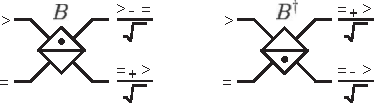
\includegraphics[width=0.75\linewidth]{figs/beamsplitter.pdf}
  \caption{(Reproduced from \autocite[289]{nielsen_2010_quantum})}
  \label{fig:beamsplitter}
\end{figure}

Applying B to a and b and applying its Hermitian conjugate results in

\begin{equation}
  \begin{aligned}\label{eq:15}
    BaB^{\dag} = a\cos\theta + b\sin\theta
  \end{aligned}
\end{equation}

\begin{equation}
  \begin{aligned}\label{eq:15}
    BbB^{\dag} = -a\sin\theta + b\cos\theta
  \end{aligned}
\end{equation}


Then apply \(B\) to a state \(\ket{\psi} = c_0\ket{01} + c_1\ket{10}\) can be seen as \(B\ket{\psi} = c_0e^{\frac{-i\theta Y}{2}}\ket{01} + c_1e^{\frac{i\theta Y}{2}}\ket{10}\). Where Y is the usual Pauli Operator Y that performs operation over the \(\hat{y}\) axis.

\begin{equation}
  \begin{aligned}\label{eq:15}
    R_y(\theta) = e^{\frac{-i\theta Y}{2}}
  \end{aligned}
\end{equation}



\section{Ion Trap}
\label{cap:ion}
The study of atomic structure and its associated energy levels provides great insight into fundamental quantum properties that can be harnessed to realize actual qubits.

\subsection{Apparatus Description}
\label{sec:apparatus_description}

To harness the quantum effects of a charged atom and enable precise control over its quantum states, it is essential to decouple the atom from any external influences. This necessitates the development of a method to confine the ion within a vacuum environment. One widely utilized approach involves the use of an electromagnetic field source to immobilize the charged particle. However, the utilization of a static electric field that can trap the particle in all directions is prohibited by Earnshaw's theorem \autocite{jones_1980_earnshaws}.

Nevertheless, there exists a viable solution that enables the confinement of the charged particle in space. By employing time-varying electrical fields, it becomes possible to generate an average force that restricts the ion's movement. This ingenious type of trap is referred to as a Paul trap \autocite{paul_1953_notizen}. At its core, a Paul trap consists of a set of electrodes capable of producing a quadrupolar electric field. This field configuration facilitates the trapping of the charged particle by exerting forces that counteract its tendency to escape along certain axes while allowing its confinement within others.

The fundamental principle underlying the operation of a Paul trap relies on the interplay between the electric fields generated by the electrodes and the motion of the charged ion. As the ion moves within the trap, its interaction with the oscillating electric fields causes it to experience a restoring force towards the trap's center. This confinement allows for stable trapping and manipulation of the ion's quantum states, which provides a good foundation for the development of a quantum computer.

There are usualy two types of Paul traps configuration, one with layout of quadrupolar electrodes that traps the ion in add three dimensions (point traps), and one with two RF trapping plus and a static eletric field that traps the ion in a plane (linear traps).
The point traps have only one point where the field is zero, thefore for multiple ions to be trapped in the same trap they need to be cooled to a point where they are almost still, or it leads to lost of fidelity.
Linear traps in general have a line where the field is zero, therefore it is possible to trap multiple ions in the same trap, and trought variation on the static field, ions can be moved and rearranged in the trap.

Figure~\ref{fig:traps} shows different geometries of Paul traps. A general description of the ion movement \autocite{leibfried_2003_quantum} can be followed from the assumption that the potential is quadratic near the trap center. The ion is then confined to a region of space where the potential is approximately harmonic. So describing the movement across each axis can be given by the Hamiltonian:

\begin{equation}
  \begin{aligned}\label{eq:ionhamilt}
    \hat{H}_t(t) = \frac{\hat{p}^{2}}{2m_I} + \frac{|e|}{2}[\Phi_{\mathrm{dc}}'' + \Phi''_{\mathrm{rf}}(\Omega_{\mathrm{rf}}t)]\hat{x}^2
  \end{aligned}
\end{equation}

\noindent In the limit when the parameter \( q_x = \frac{2|e|\Phi''_{\mathrm{rf}}}{m_I \Omega^2_{\mathrm{rf} }} \ll 1\), only a few terms are relevant, and the equations of position and momentum operators follows that of a harmonic oscillator. This analysis can be extended to the other axis, and the motional modes are orthogonal. For multiple ions in harmonic traps it becomes more complex with aditional modes of motion, but for suficient low temperatures, the ions are confined to the orthogonal harmonic modes is a good aproximation.
So with energy levels equally spaced with an frequency of \(\omega_t\), those eigenstates represent {\it center of mass} modes, and the vibrational energy of \(\hbar\omega_t\) is called a {\it phonon}.

Within the domain of ion traps, numerous sources of noise pose potential disruptions. Proximity to fluctuating electric fields, for instance, can yield unanticipated transitions in the motional state, as the electrodes fall short of ideal source conditions. Although these influences may appear inconsequential individually, their cumulative impact can impinge upon the fidelity of gate operations over time. Fortunately, most sources of noise can be managed to avert interference within the required operational time frame. By virtue of the harmonic approximation, the ions exhibit remarkable selectivity toward the frequency driving state transitions, rendering the system predominantly susceptible to noises that align closely with the motional modes frequencies.
Discussion around the many sources of noise can be found in \autocite{brownnutt_2015_iontrap}.

Given the criticality of harmonicity in bolstering the system's resilience against noise, it becomes imperative for the ions to attain a state of significant cooling to validate the harmonic approximation. This cooling mechanism is achieved through Doppler cooling. By subjecting the ion to illumination from a laser operating at a frequency slightly below the ion's resonant frequency, the ion absorbs photons and subsequently emits them in random directions, leading to a loss of momentum and energy. This iterative process continues until the ion reaches a desired level of coolness.

\noindent



\begin{figure*}
  \centering
  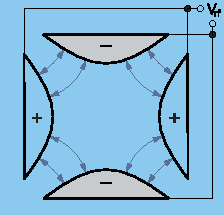
\includegraphics[height=4cm]{figs/fig1/g96736.pdf}
  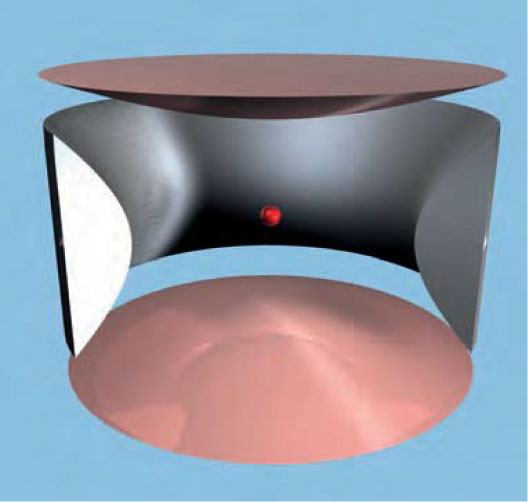
\includegraphics[height=4cm]{figs/fig1/p5_6.png}
  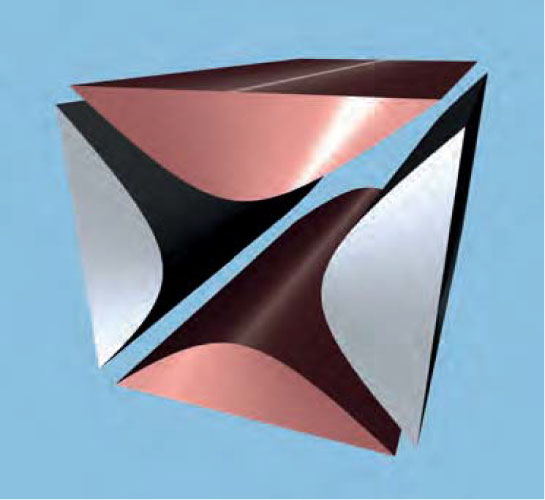
\includegraphics[height=4cm]{figs/fig1/p5_5.png}
  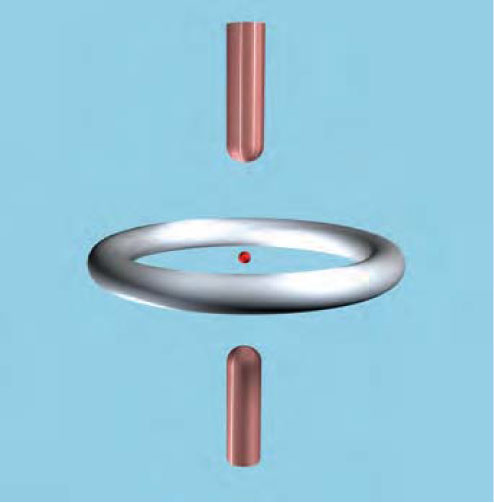
\includegraphics[height=4cm]{figs/fig1/p5_4.png}

  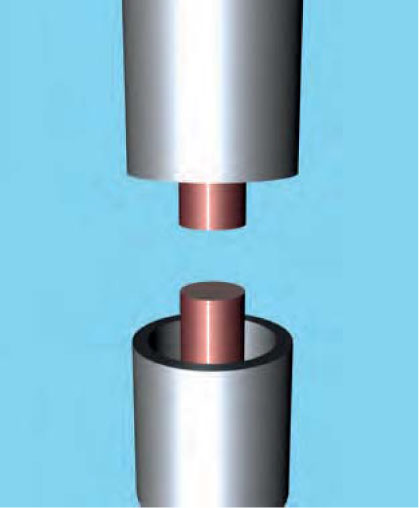
\includegraphics[height=4cm]{figs/fig1/p5_7.png}
  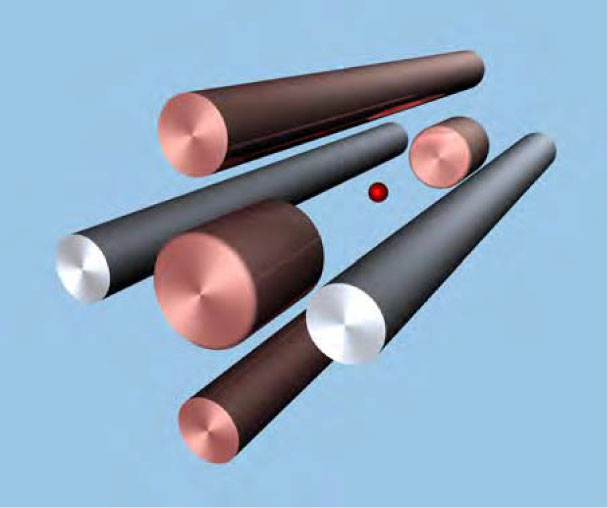
\includegraphics[height=4cm]{figs/fig1/p5_1.png}
  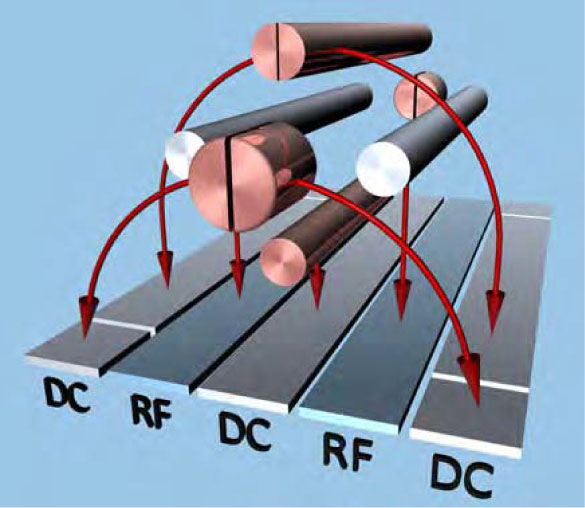
\includegraphics[height=4cm]{figs/fig1/p5_2.png}
  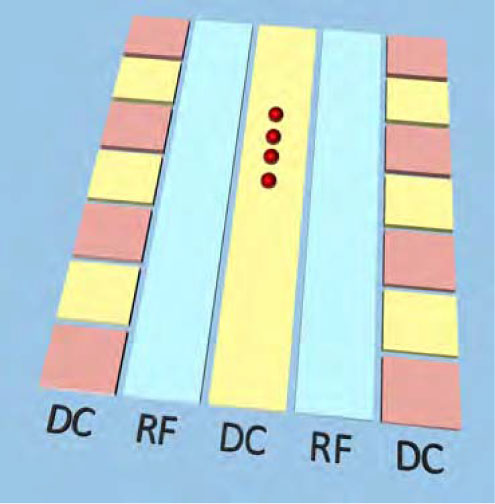
\includegraphics[height=4cm]{figs/fig1/p5_3.png}

  \caption{(Reproduced from \autocite{brownnutt_2015_iontrap}) (a) The fundamental concept of RF trapping involves the generation of quadrupolar fields that oscillate at an RF frequency. This is achieved by employing a set of (parabolic) electrodes. (b) The simplest version of the basic RF trap exhibits cylindrical symmetry and is known as the ``ring and endcap'' point-trap configuration. (c) Another simple variation of the RF trap is the translationally symmetric design, which forms a quadrupole mass filter and can be utilized as a linear trap. (d,e) Additional configurations that share the same topology as the geometry shown in (b) but exhibit slight deformations. (f) Similar topologically equivalent deformations can be applied to the geometry shown in (c), where extra endcap electrodes are incorporated to create a four-rod, linear trap. (g) By manipulating the four-rod trap in (f), it is possible to arrange all the electrodes in a single plane, resulting in a linear ``surface-electrode trap.'' (h) In a linear trap, a subset of the electrodes (depicted here using a surface-electrode trap, but applicable to other linear trap geometries as well, such as the one shown in (f)) can be segmented to enable trapping in multiple zones along the axial direction.}\label{fig:traps}
\end{figure*}

\subsection{Atomic Structure}

Trapped ions, as a means of qubit representation, rely on the utilization of internal electronic states of the ion to embody the qubit states \(\ket{0}\) and \(\ket{1}\). Trapped-ion qubits can be broadly classified into four distinct categories: hyperfine qubits, where the qubit states emerge from hyperfine states of the ion, distinguished by an energy splitting in the order of gigahertz; Zeeman qubits, where the qubit states stem from magnetic sublevels, segregated by an  applied field, typically exhibiting frequencies in the tens of megahertz range; fine structure qubits, where the qubit states inhabit fine structure levels, characterized by separations on the order of tens of terahertz; and optical qubits, where the qubit states manifest through an optical transition, generally featuring frequencies in the hundreds of terahertz.~\autocite{mattos_2023_estudo}

The origin of these states can be traced back to the combination of the total angular momentum J, which comprises the electron spin S and the orbital angular momentum L. This phenomenon finds comprehensive explanation in physics through the concept known as the {\it addition of angular momenta.} This theoretical framework offers a systematic approach to deduce the atomic structure by amalgamating the individual angular momenta Hamiltonians.

The current objective of our study does not involve the selection of a specific system; instead, it aims to present a comprehensive overview of the field in a more generalized manner. Hence, we shall refrain from delving into the intricate details of the atomic structure pertaining to any particular system. Rather, our intention is to provide a broader perspective on the subject. The choice of eigenstates for qubit states, while system-dependent, typically centers around the lowest non-degenerate energy levels, enabling individual addressing through the utilization of lasers.

\subsection{State preparation}

In trapped ion systems, the preparation of the ion register's internal state and motional state plays a crucial role in enabling subsequent quantum operations. High-fidelity initial state preparation must be performed after each experimental realization. Various operations, such as Doppler cooling and state measurement, can result in ions occupying internal states beyond the qubit subspace. Thus, optical pumping is employed to either prepare the desired initial state or an intermediate state that can be coupled to the initial state with high fidelity. Optical pumping schemes utilize photon absorption and emission selection rules to effectively confine quantum state amplitudes to a single state through repeated absorption and emission cycles. Although off-resonant excitation and residual branching can limit state preparation fidelity, errors on the scale of \(10^{-4}\) can be achieved~\autocite{harty_2014_highfidelity}.

Controlling the motional state of the ion register is also crucial. Laser-based Doppler cooling is utilized to rapidly reduce the ion temperature to millikelvin scales. However, for trapping frequencies typically employed in quantum processing experiments, this cooling method leaves the ions in a thermal distribution spanning multiple motional states. Resolved sideband cooling is an efficient technique for further reducing the motional state occupation of the ion register when addressing small numbers of ions or controlling a few motional modes~\autocite{monroe_1995_demonstration}. By absorbing photons tuned to specific motional modes' narrow red sideband transitions, the state occupation of those modes is reduced. Subsequent state quenching and spontaneous decay maintain the motional state in the Lamb-Dicke regime and permit the cooling cycle to repeat. However, resolved sideband cooling can become slow and impractical for large ion chains with numerous motional modes due to the need for repeated resonant addressing of weak transitions.

An alternative cooling approach involves employing electromagnetic induced transparency (EIT) to alter the ion register's light absorption profile. By carefully selecting laser frequencies and polarizations, a \( \lambda \)-level scheme can be utilized to inhibit photon scattering on blue sideband transitions and preferentially reduce the motional state occupation. This technique was initially applied to single ions but has been extended to efficiently cool longer chains and simultaneously address multiple motional modes~\autocite{lechner_2016_electromagneticallyinducedtransparency}.

\subsection{Quantum Gates}
For a quantum computer to be able to perform useful computations, it must be able to perform a universal set of quantum gates.

Trapped-ion qubits exhibit different types depending on their internal states and transition frequencies. Hyperfine qubits utilize two hyperfine states with gigahertz separations as the \(\ket{0}\) and \(\ket{1}\) states. Single-qubit gates for hyperfine qubits can be performed using microwaves or Raman transitions. On the other hand, optical qubits employ a metastable excited state with optical transition frequencies exceeding 100 terahertz, enabling single-qubit gates with a resonant laser.

Optical qubits typically utilize two internal states separated by an electric quadrupole \(S \to D\)  transition. Although these qubits have longer lifetimes, coherence times are limited by T2 constraints due to laser phase noise and optical path length fluctuations. Despite their potential, optical qubits have not been extensively utilized. However, they hold promise for future quantum computing endeavors, especially with the recent development of millihertz-class lasers for optical clocks.

Hyperfine qubits can be subjected to laser-based gates employing stimulated Raman coupling. This approach involves two laser beams detuned from a dipole-allowed transition and each other by the splitting of the \(\ket{0}\) and \(\ket{1}\) states. The precision control of the difference frequency between the Raman beams allows for coherent operations. Additionally, direct microwave drives at gigahertz transition frequencies can implement gates on hyperfine qubits by coupling to the ion's magnetic dipole. While individual addressability is challenging with microwave radiation, microfabricated chip traps integrated with current-carrying wires enable near-field microwave transitions. By selectively moving ions in and out of microwave zones, gates can be implemented on one ion at a time in a multi-ion system, mitigating crosstalk within the chip's zones.


For multiple qubit gates, one widely employed method is the entangling gate devised by Cirac and Zoller (CZ gate)~\autocite{cirac_1995_quantum}. This approach has stood the test of time and continues to serve as the foundation for modern techniques. The CZ gate capitalizes on the collective behavior of ions' shared motional modes, utilizing them as a conduit for transferring quantum information among the qubits.

A sequence of carefully tailored laser pulses or microwave fields is applied to the ions, exploiting their interaction with the electromagnetic field. These external fields induce controlled interactions between the ions' internal states and their shared motional modes.
As the qubits interact with the motional modes, their internal states become entangled.

\subsection{Sources of noise}

Regarding the sources of noise, numerous elements can influence the efficacy of a trapped-ion quantum computer. As elucidated in Section~\ref{sec:apparatus_description}, there are various factors that contribute to the system's decoherence. A comprehensive exploration of the noise sources in ion-traps can be found in the work by Brownnutt (2015)\autocite{brownnutt_2015_iontrap}, offering valuable insights into this domain.

\section{Solid State: Superconducting Qubits}
\label{cap:superconductor}

A notable platform for constructing a multi-qubit quantum processor revolves around superconducting qubits. These qubits employ the quantum degrees of freedom found within nanofabricated, anharmonic oscillators built from superconducting circuit components. Div'rging from alternative platforms, wherein quantum information is encoded within natural microscopic quantum systems, superconducting qubits exhibit a macroscopic scale and are lithographically defined.

A striking characteristic of superconducting qubits resides in their energy-level spectra, which are determined by circuit element parameters. This configurability enables the design of ``atom-like'' energy spectra with specific desired properties. Hence, superconducting qubits are frequently hailed as artificial atoms, presenting a diverse parameter space that encompasses a myriad of qubit properties and operational modes. They offer a predictable performance with respect to transition frequencies, anharmonicity, and intricacy, providing a great oportunity to explore qubit implementations.

\subsection{Transmon qubit}
A quantum system is governed by the Schrödinger equation (postulate ~\ref{post:schroedinger}), which describes the time evolution of the system's state vector. As discussed in Section~\ref{sec:physical_properties}, the Hamiltonian governs the time evolution trough the unitary operator \(U\). So the first step to determine the Hamiltonian is to consider its classical counterpart. We will consider only the time-independent Hamiltonian as it provides a useful enough description of the system.

To understand the dynamics of a superconducting qubit circuit, it is customary to commence with the classical portrayal of a linear LC resonant circuit. Within this configuration, energy undergoes oscillations between electrical energy stored in the capacitor C and magnetic energy stored in the inductor L. For later analogies, we will arbitrarily associate the electrical energy with the ``kinetic energy'' and the magnetic energy with the ``potential energy'' of the oscillator. The energy present in each element at any given moment is contingent upon its current and voltage:

\begin{equation}
  E(t) = \int_{-\infty}^{t} I(t')V(t')dt'
\end{equation}

We can represent the circuit elements in terms of a generalized circuit coodinate, the {\it flux}, defined as the time integral of the voltage across the component:
\begin{equation}
  \Phi(t) = \int_{-\infty}^{t} V(t')dt'
\end{equation}

Combining the equations with the relations \( V = \frac{dI}{dt} \) and \( I = C \frac{dV}{dt}\), it is possible to write the energy of the capacitor and inductor in terms of the flux:
\begin{eqnarray}
  \mathcal{T}_C = \frac{1}{2}C\dot\Phi^2\label{eq:tc} \\
  \mathcal{U}_L = \frac{1}{2L}\Phi^2\label{eq:ul}
\end{eqnarray}

\noindent To find the hamiltonian we can follow the classical mechanics Lagrange-Hamiltonian formulation. The Lagrangian, a key concept in classical mechanics, arises as the discrepancy between the kinetic and potential energy components. Consequently, we can express the Lagrangian using the equations~\ref{eq:tc} and~\ref{eq:ul}.


\begin{equation}
  \mathcal{L} = \mathcal{T}_C - \mathcal{U}_L = \frac{1}{2}C\dot\Phi^2 - \frac{1}{2L}\Phi^2
\end{equation}

\noindent And we can now derive the Hamiltonian by finding the momentum conjugate to the flux, which is the charge \( Q = C\dot\Phi \). The Hamiltonian is then given by:
\begin{equation}
  Q\dot\Phi-\mathcal{L} = \frac{Q^2}{2C} + \frac{\Phi^2}{2L} = \frac{1}{2}CV^2 + \frac{1}{2}LI^2
\end{equation}

\noindent This Hamiltonian is analogous as the one for a harmonic oscillator, with mass \(C\) and resonant frequency \(\frac{1}{\sqrt{LC} }\).

To probmote charge and flux to quantum operators, we can use the commutation relation \( [\hat\Phi, \hat Q] = i\hbar \). In a LC circuit, both the capacitor and inductor are linear components, so the Hamiltonian is then given by:
\begin{equation}
  H = 4E_C n^2 = \frac{1}{2}E_L\phi^2
\end{equation}
\noindent where \(\phi = 2\pi\frac{\Phi}{\Phi_0}\) is the reduced flux, \(n = \frac{Q}{2e}\) is the reduced charge, \(E_C = \frac{e^2}{2C}\) is the charging energy, \(E_L = \frac{\Phi_0^2}{4\pi^2L}\) is the inductive energy, and \(\Phi_0 = \frac{h}{2e}\) is the superconducting magnetic flux quantum.

This Hamiltonian is identical to the quantum harmonic oscilator, and can be written in terms of the raising and lowering operators \(a^\dagger\) and \(a\):
\begin{equation}
  H = \hbar\omega(a^\dagger a + \frac{1}{2})
\end{equation}
\noindent Aditional discussion over the correspondence can be found at \autocite{krantz_2019_a}, but we will limit ourselves to this brief overview.

\begin{figure}[t]
  \centering
  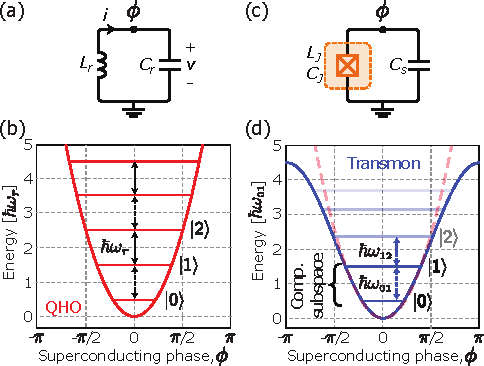
\includegraphics[width=0.75\linewidth]{figs/circuits.pdf}
  \caption{(Reproduced from \autocite{krantz_2019_a})
    (a) Illustrated here is the circuit diagram for a parallel LC-oscillator, also known as a quantum harmonic oscillator (QHO). The inductance \(L\) and capacitance \(C\) are connected in parallel. The superconducting phase on the island is represented as \( \phi \) , with reference to ground as the zero point.
    (b) The energy potential graph depicts the QHO, wherein the energy levels are uniformly spaced, separated by approximately \(\omega_r\).
    (c) Shown is a Josephson qubit circuit, featuring a nonlinear inductance \(L_J\)  (depicted within the dashed orange box) that is coupled with a capacitance \(C_S\).
    (d) The Josephson inductance modifies the quadratic energy potential (illustrated by the dashed red curve) into a sinusoidal shape (depicted by the solid blue curve). As a result, the energy levels become non-uniformly spaced. This characteristic enables the isolation of the two lowest energy levels, denoted as \(\ket{0}\) and \(\ket{1}\), forming a computational subspace. The energy separation between these levels is approximately \(\omega_{01}\), distinct from \(\omega_{12}\).}
  \label{fig:circuits}
\end{figure}

One notable aspect to observe here is the linearity exhibited by the quantum harmonic oscillator, as seen if Figure~\ref{fig:circuits}.a. In the case of eigenstates associated with the number operator \((N=a^\dagger a)\), the energy levels of this system are evenly spaced by a factor of \( \hbar\omega \). However, this presents a constraint as we require the ability to manipulate single qubits with different transition frequencies.

To overcome this limitation, we can introduce a anharmonicity (non-linearity) to the system. This can be achieved by incorporating a shunting capacitor in parallel with the Josephson junction~\autocite{josephson_1962_possible}\autocite{josephson_1964_coupled}. This particular configuration gives rise to what is known as a {\it transmon} qubit, which is governed by the modified Hamiltonian:

\begin{equation}
  H = 4E_C n^2 - E_J cos(\phi)
\end{equation}

\noindent where \(E_C = \frac{e^2}{2C_\Sigma}\) and \(C_\Sigma = C_S+C_J\). So with the Josephson junction, the energy potential is no longer quadratic, but rather sinusoidal, as seen in Figure~\ref{fig:circuits}.d. This results in a non-uniform spacing between energy levels, which allows for the isolation of the two lowest energy levels, forming a computational subspace. The energy separation between these levels is approximately \(\omega_{01}\), distinct from \(\omega_{12}\), thus not causing unwanted transitions. We now have access to a individually addressable two-level quantum system.

We will not discuss in details here, but one choice that comes with this system is the \(\frac{E_J}{E_C}\) ratio. There are two regimes to choose, the \(E_J \leq E_C\) or the \(E_J \gg E_C\). The current preferential regime is the later, as it is more robust to charge noise, and has a longer coherence time~\autocite{krantz_2019_a}.

\subsection{Adressing qubits}

In order to implement single-qubit gates, a microwave source, commonly referred to as the "qubit drive," is coupled with the transmon qubit. This coupling exploits the anharmonicity produced by the Josephson junction. For a more in-depth understanding of this particular interaction, details can be found in the references~\autocite{girvin_circuit}\autocite{krantz_2019_a}\autocite{gustavsson_2012_driven}\autocite{bertet_2006_parametric}. However, for the purpose of this overview, we will provide a brief summary of the results.

The driving Hamiltonian for a microwave pulse interacting with a  single superconducting qubit in a frame rotating at the drive frequency \(\omega_q\) is given by:

\begin{equation}
  \tilde H_d = -\frac{\Omega}{2}V_0 s(t) \begin{pmatrix}
    0                             & e^{i(\delta\omega t + \phi)} \\
    e^{-i(\delta\omega t + \phi)} & 0
  \end{pmatrix}
\end{equation}

The pulse is then described by the function \(s(t)\), which is the envelope of the pulse, and \(\phi\) is the phase of the pulse. The parameter \(\Omega\) is the Rabi frequency, which is proportional to the amplitude of the pulse. The parameter \(V_0\) is the coupling strength between the qubit and the drive, and is proportional to the amplitude of the drive.

As an example we can imagine a pulse at the quit frequency, so that \(\delta\omega = 0\). In this case, the Hamiltonian becomes:

\begin{equation}
  \tilde H_d = - \frac{\Omega}{2}V_0 s(t)(I\sigma_s+Q\sigma_y)
\end{equation}

\noindent showing that an in-phase pulse correspond to a rotation around the x-axis, and a out-of-phase pulse correspond to a rotation around the y-axis.

For transmon-like superconducting qubit architecture, the available two-qubit gates can be broadly classified into two distinct families, as previously discussed. The first family encompasses gates that necessitate local magnetic fields to tune the transition frequency of qubits. On the other hand, the second family comprises all-microwave control gates. However, it is worth noting that there exist hybrid schemes that amalgamate elements from both categories.
iSWAP gates has been demonstrated to work with a high fidelity~\autocite{sung_2021_realization}, and in combination with another single-qubit gates, it can reproduce a C-NOT, and generate a complete set of universal gates~\autocite{krantz_2019_a}.

\subsection{Sources of noise}
Various sources of noise can impact the performance and fidelity of superconducting qubits.

Within the surrounding environment, thermal fluctuations manifest as random electromagnetic fields and thermal excitations. These fluctuations introduce noise, leading to energy dissipation and potential errors in the qubit's state.

Superconducting qubits are susceptible to fluctuations in the magnetic flux passing through their loops. These fluctuations arise from interactions between the qubit and its magnetic surroundings, encompassing stray magnetic fields or material defects. Flux noise engenders random variations in the qubit's energy levels, ultimately causing decoherence and errors.

Proximity to charge fluctuations can impact the performance of superconducting qubits. Charge noise emanates from nearby charge traps or impurities within the substrate or dielectric layers. These fluctuations can perturb the qubit's energy levels, thereby introducing errors during qubit operations.

\section{Comparative Analysis}
\label{sec:comparative}

A comparative analysis of quantum computer architectures plays a crucial role in evaluating and understanding the capabilities and limitations of these systems. Understanding the differences between the available architectures is critical to directing future development and identifying the most promising technologies for practical applications. By far, the superconducting qubit architecture is the predominant and most common architecture of today's quantum computers. This is mainly due to the technological maturity of the area and the in-depth understanding of the properties of superconducting materials. Solid-state physics is an area on the rise and is one of the areas that has grown the most, if not the most, in recent years. We can cite as highlights of the architecture of superconducting qubits the scalability of these systems, that is, the ability to form larger circuits, increase the number of qubits efficiently, generally operates at higher frequencies and work with multi-gates. Devoret, Wallraff and Martinis also highlights some qualities of this architecture in their article ``Superconducting Qubits: A Short Review'':~\autocite{devoret_2004_superconducting}

\begin{enumerate}
  \item \emph{Coherence quality factors \(Q_\phi = T_\phi\omega_{01}\) can attain at least \(2x10^4\) }
  \item \emph{Readout and reset fidelity can be greater than 95\%}
  \item \emph{All states on the Bloch sphere can be addressed}
  \item \emph{ Spin echo techniques can null out low frequency drift of offset charges}
  \item \emph{Two qubits can be coupled and RF pulses can implement gate operation.}
  \item \emph{A qubit can be fabricated using only optical lithography techniques.}
\end{enumerate}


The main rival of the superconducting qubit architecture is certainly the ion trap architecture. Some advantages of ion trap architecture over superconducting qubits is that the ion trap system features superior qubits and reconfigurable connections, the construction and reading of results with greater fidelity. Moving on to a more practical analysis, the experimental results comparing these two models in a research published in 2017(``Experimental comparison of two quantum computing architectures'') pointed to an advantage in favor of the ion trap model, demonstrating superior fidelity in the states and greater probability of success in the implementation of diverse circuits and quantum gates. One of the reasons for this result pointed out in the article is due to the topology of the connections, supporting the idea that quantum computer applications and hardware should be codesigned.~\autocite{linke_2017_experimental}


The photonic model, in contrast to the other two, appears little in the realization of well-established quantum computers, some companies that have bet on this architecture for the future are PsiQuantum and Xanadu but today this model is more speculative and a promise for the near future. The reason why the photonic model is currently difficult to perform is because the interaction between photons is very weak and as evidenced by the comparison between ion trap and superconducting qubits the fact that the ion trap was fully-connected was a key factor in its advantage over the superconducting model.

\begin{table}[]
  \begin{tabular}{lllllll}
    \multicolumn{1}{c}{\textbf{Connectivity}} & \multicolumn{3}{c}{\textbf{Star shaped}}     & \multicolumn{3}{c}{\textbf{Connectivity}}                              \\
    \multicolumn{1}{c}{\textbf{Hardware}}     & \multicolumn{3}{c}{\textbf{Superconducting}} & \multicolumn{3}{c}{\textbf{Ion trap}}                                  \\
    Sucess probability\%                      & Obs                                          & Rand                                      & Sys & Obs     & Rand & Sys \\
    Margolus                                  & 74.1(7)                                      & 82                                        & 75  & 90.1(2) & 91   & 81  \\
    Toffoli                                   & 52.6(8)                                      & 78                                        & 59  & 85.0(2) & 89   & 78  \\
    Bernstein-Vazirani                        & 72.8(5)                                      & 80                                        & 74  & 85.1(1) & 90   & 77  \\
    Hidden Shift                              & 35.1(6)                                      & 75                                        & 52  & 77.1(2) & 86   & 57  \\
  \end{tabular}
  \caption{
    Reproduced from \autocite[6]{linke_2017_experimental} Summary of the achieved success probabilities for
    the implemented circuits, in percent.
  }
\end{table}

\section{Conclusion}

In summary, the physical implementation of quantum computers presents a landscape of both promising opportunities and formidable challenges. Quantum mechanics, with its foundational postulates, establishes the framework for comprehending the intricate behavior of quantum systems. The prerequisites for a viable quantum computer, as outlined by DiVincenzo, encompass a scalable physical system housing well-characterized qubits, the capacity to initialize and manipulate qubits, extended decoherence times, a universal set of quantum gates, and qubit-specific measurement capabilities.

Numerous approaches have been explored for the realization of quantum computers, with photonics-based platforms, trapped ions, and superconducting circuits emerging as leading contenders. Each avenue possesses its unique advantages and disadvantages. Notably, superconducting circuits have garnered significant attention owing to their potential for sustaining prolonged qubit coherence and enabling the implementation of multi-qubit gates.

Nevertheless, the construction of large-scale quantum architectures remains a formidable undertaking, primarily due to the fragility of qubits and the imperative of upholding quantum coherence amidst environmental disturbances. Challenges encompass decoherence, gate operation durations, and the reliable transmission of qubits, necessitating focused attention to achieve practical and scalable quantum computing.

Despite those obstacles, the relentless progress in hardware development, error correction techniques, and algorithmic enhancements presents a hopeful outlook for the trajectory of quantum computing. As dedicated researchers and engineers persistently push the frontiers of quantum technology, the transformative power of quantum computing emerges as a pivotal force poised to revolutionize diverse domains such as cryptography, optimization, simulation, and machine learning. The expedition toward unlocking the complete potential of quantum computers stands as an ongoing pursuit that captivates the scientific community and industry alike, forging a path towards a future embellished with unparalleled computational capacities.

\printendnotes

\printbibliography

\appendix

\end{document}